% \pagestyle{empty}
% \pagestyle{headings}

\usepackage{fancyhdr}
% \pagestyle{fancy} % Enable the fancy page style




\fancypagestyle{styleDigital}{
  \fancyhf{}% Clear header/footer
  % O = odd; E = even; L/R/C = left/right/center
  \fancyhead[RO, RE]{\myArticleTitle}
  \fancyhead[LO, LE]{\myPrintOrDigitalMarker}
  \fancyhead[CO, CE]{
    % \verticalCenterIcon{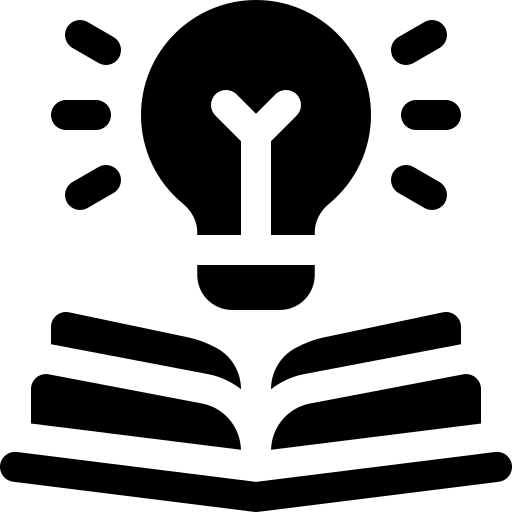
\includegraphics[scale=0.05]{../../articles_common_files/assets/icons/placeholder.png}}
  }
  % \fancyhead[CO, CE]{\textcolor{myColorPrimary}{\hyperlink{toc}{\leftmark}}}
  \fancyfoot[RO, RE]{
    \textcolor{myColorPrimary}{
      % \hyperlink{title}{\myCiteEntry{\myarticleKey}{author}}
    }
    \myAbsolutePagination
  }
  \fancyfoot[CE, CO]{
    \myRelativePagination
  }
}

%%% DEFINE ANOTHER STYLE BASED ON THIS ONE
\fancypagestyle{styleDigital-NoPage}[styleDigital]{
\fancyfoot[]{} % empty footer
\fancyfoot[RO, RE]{\myAbsolutePagination}
\fancyfoot[LO, LE]{\isDraft{\color{myColorWarning}page without pagination in final v.}{}}
}



\fancypagestyle{stylePrint}{
  \fancyhf{}% Clear header/footer
  % O = odd; E = even; L/R/C = left/right/center
  % HEAD
  \fancyhead[RO, LE]{\myArticleTitle}
  % \fancyhead[LO, RE]{\textcolor{myColorPrimary}{\hyperlink{toc}{\leftmark}}}

  % FOOT
  \fancyfoot[LO, RE]{
    % \textcolor{myColorPrimary}{\hyperlink{title}{\myCiteEntry{\myarticleKey}{author}}}
    \myAbsolutePagination
     }
  \fancyfoot[RO, LE]{
    \textcolor{myColorPrimary}{\myRelativePagination}
    }
  \fancyfoot[CO]{
    % \verticalCenterIcon{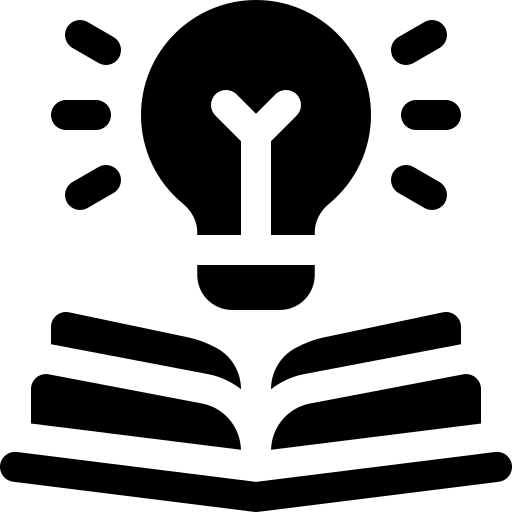
\includegraphics[scale=0.05]{../../articles_common_files/assets/icons/placeholder.png}}
    \isDraft{\textcolor{myColorWarning}{ODD (RIGHT)}{}}
  }
  \fancyfoot[CE]{
    % \verticalCenterIcon{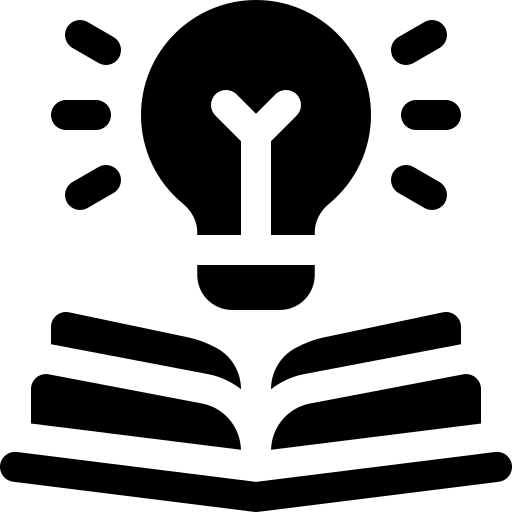
\includegraphics[scale=0.05]{../../articles_common_files/assets/icons/placeholder.png}}
    \isDraft{\textcolor{myColorWarning}{EVEN (LEFT)}{}}
  }
}

%%% DEFINE ANOTHER STYLE BASED ON THIS ONE
\fancypagestyle{stylePrint-NoPage}[stylePrint]{
  \fancyfoot[LO,RE, RO, LE]{} % empty footer
  \fancyfoot[LO, RE]{\myAbsolutePagination}
  \fancyfoot[RO, LE]{\isDraft{\color{myColorWarning}page without pagination in final v.}{}}
}


\newcommand{\verticalCenterIcon}[1]{
    \raisebox{-0.5\height}{%center vertically in line
    \scalebox{-1}[1]{%horizontal flipping
      #1
    }
  }
}

%%% Relative pagination (within article)
\newcommand{\myRelativePagination}{%
  \isDraft
  {\hyperlink{toc}{\textcolor{myGrayMed}{\thepage}} \textcolor{myColorPrimary}{out of\totalPagesInArticleBody}}%
  {
    \textcolor{myColorPrimary}{\hyperlink{toc}{\thepage}}%
  }
}

%%% Absolute pagination (whole document)
\newcommand{\myAbsolutePagination}{%
  \isDraft{\textcolor{myColorPrimary}{Absolute page: \textcolor{myGrayMed}{\abspagenumber}/\ztotpages}}{}%
}

%%% Article title
\newcommand{\myArticleTitle}{%
  \hyperlink{\myarticleKey}{\textcolor{myColorPrimary}{\setTitleFont\citefield{\myarticleKey}{title}}}%
}

%%% Print/Digital marker
\newcommand{\myPrintOrDigitalMarker}{%
  \isDraft{%
  \color{myColorWarning}\isPrint{PRINT VERSION}{DIGITAL VERSION}
  }{}
}



% to exclude "chapter #" from footer:
% \renewcommand{\chaptermark}[1]{\markboth{\MakeUppercase{#1}}{}} %remove \makeuppercase{} to keep it normal case

% change ruler style and color
\renewcommand{\headrule}{\hbox to\headwidth{\color{myColorPrimary}\leaders\hrule height \headrulewidth\hfill}}
\renewcommand{\footrule}{\hbox to\headwidth{\color{myColorPrimary}\leaders\hrule height \headrulewidth\hfill}}

% set ruler dimensions
\renewcommand{\headrulewidth}{0pt}
\renewcommand{\footrulewidth}{0pt}
\setlength{\headheight}{15pt}


\fancyheadoffset{0cm}
